\documentclass[a4paper]{article}
\usepackage[utf8]{inputenc}
\usepackage{graphicx}
\usepackage{amsmath}
\usepackage[bottom=2.0cm,top=2.0cm,left=2.0cm,right=2.0cm]{geometry}
\usepackage{indentfirst}
\usepackage{hyperref}
\usepackage{karnaugh-map}
\setlength{\parindent}{0pt}
\parskip = \baselineskip
\hypersetup{colorlinks,citecolor=black,filecolor=black,linkcolor=black,urlcolor=black}

\begin{document}

\begin{titlepage}
	\begin{center}
		\begin{figure}[htb!]
            \centering
            
\includegraphics[height=4.5cm]{images/zjuuiuc.png}
		\end{figure}
        \vspace{10pt} % {-2.5cm}
        
        \LARGE{\textbf{ECE385}}\\
        \vspace{5pt}
        \Large{Fall 2021}\\
        \vspace{5pt}
        \Large{Lab Report}\\
        
        \vspace{100pt}
        
        %\LARGE{LAB 02}\\ 
        \huge{\textbf{Final Project Proposal}}\\ 
        
        \vspace{150pt}
        
        % \hfill Group: 11 \\
        
        \vspace{10pt} 
        \hfill Liu Peiyuan \hspace{10pt} ID: 3190112158\\
        \vspace{10pt}
        \hfill Song Yifei \hspace{10pt} ID: 3190110099\\
        \vspace{10pt}
        \hfill Lab Section: \hspace{10pt} D225-Morning\\
        \vspace{10pt}
        \hfill TA: \hspace{10pt} Wang Lianjie\\
        % \hfill Galileo Galilei \hspace{20pt} Mat: xxxxxx  \\
        % \hfill Albert Einstein \hspace{20pt} Mat: xxxxxx\\
        % \vspace{25pt}
        % \hfill \underline{Professor:}\\
        % \hfill Jairo Rocha\\
        \vspace{\fill}
        \LARGE \bf{December 2, 2021}
	\end{center}
\end{titlepage}

\newpage


\pagenumbering{arabic}
\large
% Part of Introduction
\section{Idea \& Overview}
We propose to design and implement the \textbf{Fireboy and Watergirl} game on the Altera DE2 board. Using SystemVerilog, we will implement the fireboy and watergirl, a color mapper, some obstacles displayed on a VGA monitor. We will also utilize components such as RAM, system bus, FPGA, speaker, and keyboard to make the game more functional. 
We will use the NIOS II CPU that is similar to what we implemented on the USB interface for lab 8 to allow user input from the keyboard or controller to control the motion of two characters, using C code. The plan is to implement a fully functional adventure game.
\section{Block Diagram}
\begin{figure}[ht]
    \centering
    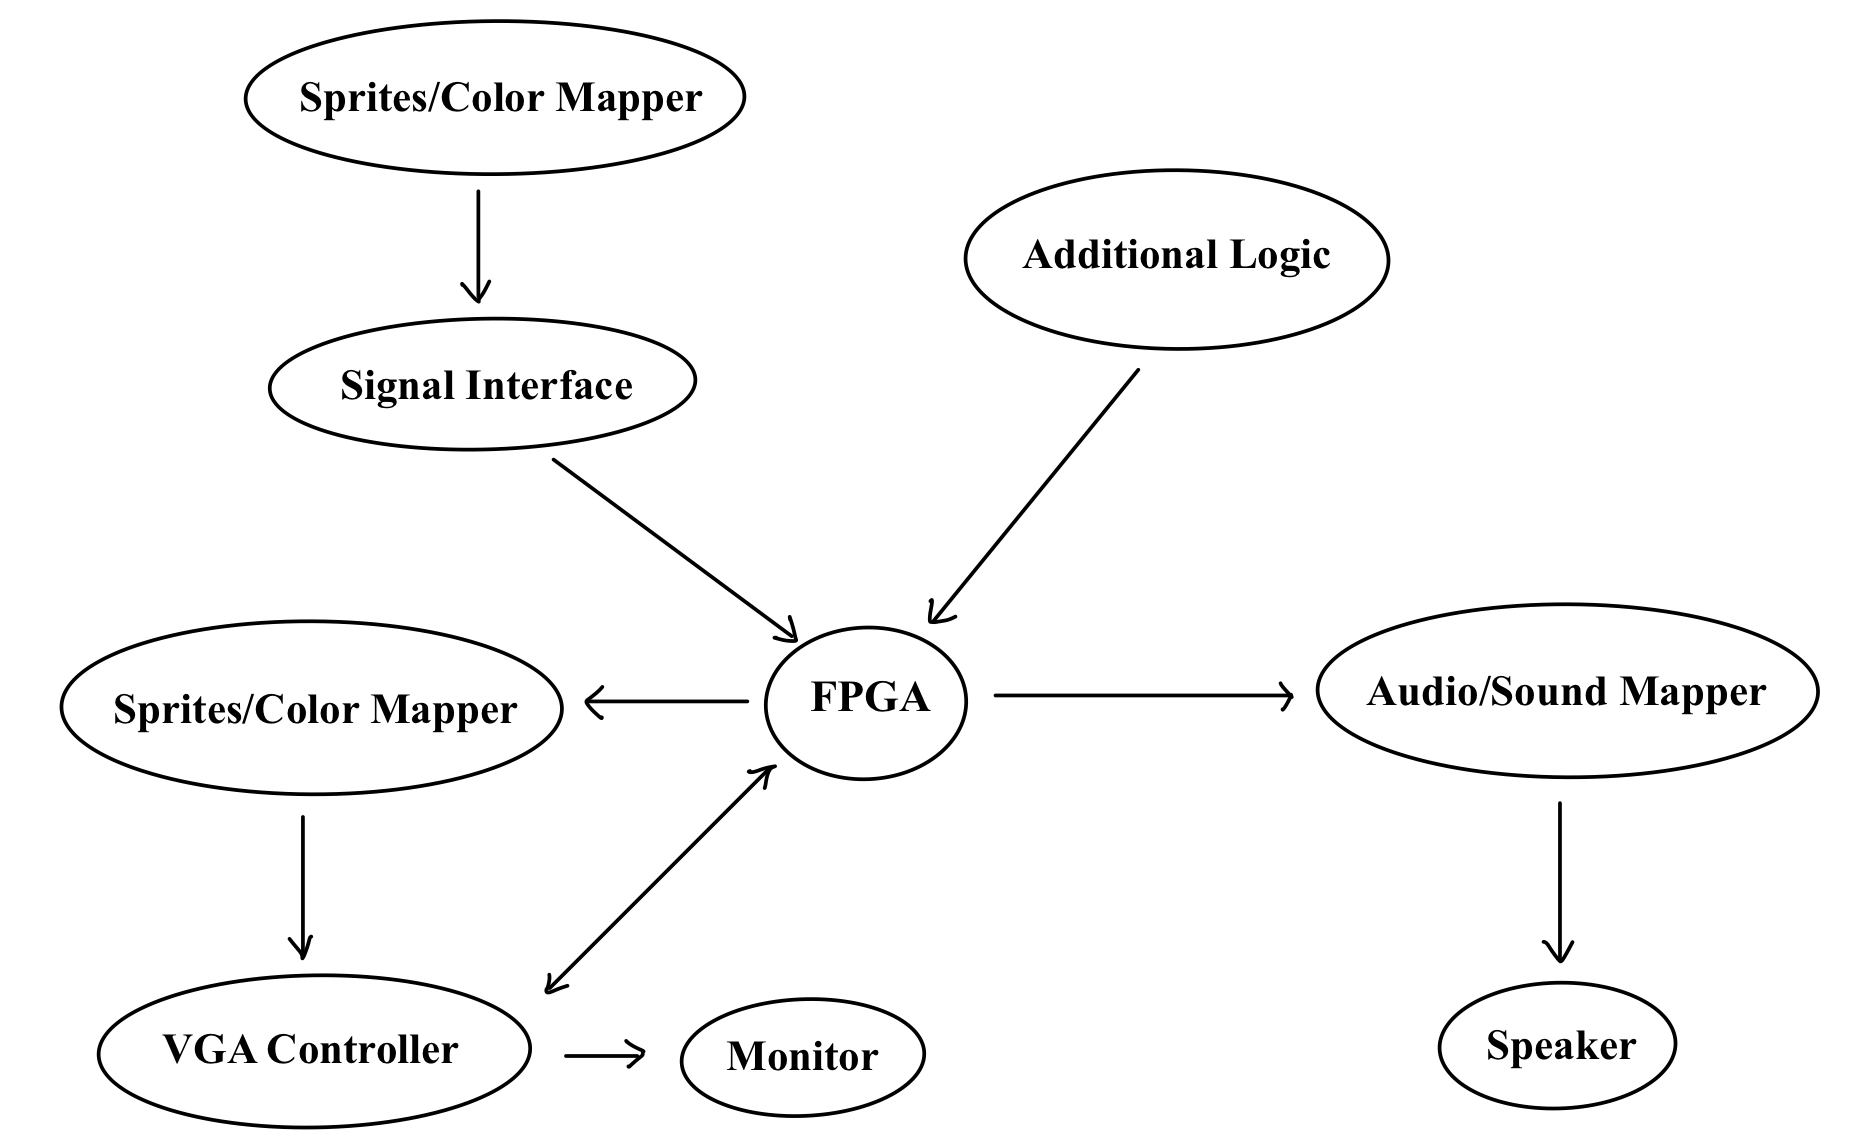
\includegraphics[width = 0.95\textwidth]{images/block diagram.jpeg}
    \caption{Block Diagram}
\end{figure}
\section{List of Features}
\subsection{Baseline Feature}
For baseline edition, we are going to implement a single-player version of the first level of \textbf{Fireboy and Watergirl}. There will be a start screen at the beginning of the whole game. 
The end screen can either be “Game Over” which lets the player choose from retrying or exiting, or “Success” which congratulates the player for a good game. 
We plan to design three kinds of movement for the player which include moving left, moving right and jump. These movements are controlled by the player through the USB input from the keyboard (A, W, D). 
For the interface, we plan to use NIOS II for the keyboard to determine the movement of the character. Also, the character can automatically push the box or handler when directly touching it and push the button on the ground by standing on it. 
We will also set up the frame of the ground, ceil and wall which could stop the character from moving out of the map. The number of diamonds collected by the player will be shown on the hex display of the DE2 board. 
The character starts running from the bottom and ends with success at the top gates. Falling into the toxic liquid will be considered a failure(death).

\subsection{Additional Feature}
The above descriptions are about the simplified version of the original \textbf{Fireboy and Watergirl}. Suppose we can manage to finish the baseline features in time. We plan to optimize the game by adding more features and approach the original version. 
Based on the above design of basic movements, judging logic (push box, handler or button), we plan to add background sound and notification sounds to the game. For instance, there will be extra sound when the character falls into the toxic liquid or 
enter the final gates. Furthermore, we will try to add another player (watergirl) to the game which is controlled with arrow keys (up, left, right).

\begin{figure}[ht]
    \centering
    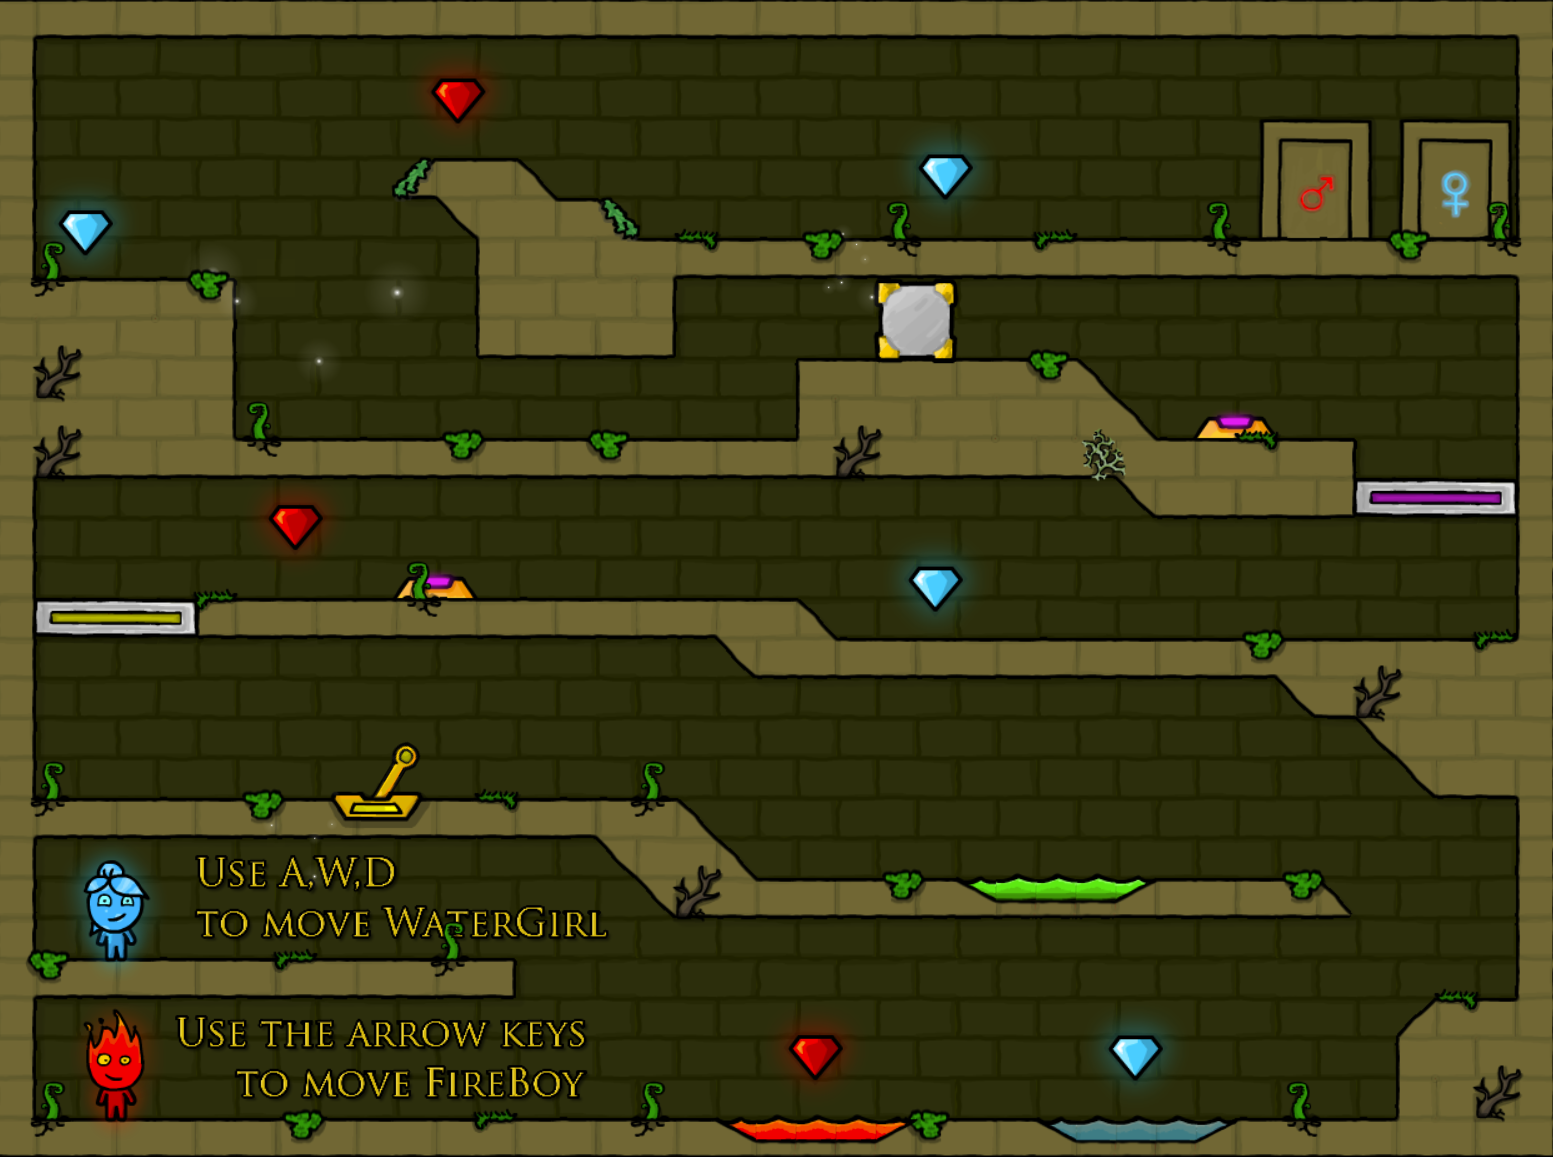
\includegraphics[width = 0.95\textwidth]{images/1.png}
    \caption{Illustration of the Interface}
\end{figure}

\section{Expected Difficulty and Justification}
From our perspective of view, the baseline version of the game should be assigned with 5-7 points. We need to set up the background and basic frame of map by collecting the image sources from the game and modifying the sv and C code as lab8. 
Also we need to map keyboard input to the movement of the character through modifying sv code. Other features in the baseline version will be mostly implemented in C code, such as the judging logic, free-fall motion, diamond counting, etc. 
These small features will make the project more complex than the Tetris. Therefore, we propose that the baseline version should be assigned more than 5 points. Considering the complexity of designing Apple IIe computer running graphical games (9 points), 
the baseline version should be assigned less than 9 points. Consequently, the expectation falls in 5-7 points which will kind of fluctuate as we adjust our design dynamically in the process of coding. Apart from the baseline version, we may get extra 
points by adding features to the previous version. Such features include adding background sound and notification sounds but not limited to that. If there is still time left, we may try to upgrade the game into a two-player version. 

\section{Proposed Timeline}
Based on the 5 weeks we are assigned to work on this project, our ideal schedule will be as follows:
\par \textbf{Week 1:} Understand and plan what is needed for the game. This includes but not limited to fireboy, obstacles, motion, etc. We will need to have defining PIO blocks for Qsys and implementing boundaries for objects.

\par \textbf{Week 2:} ​Start the groundwork for the baseline of the game. We will implement the fireboy, the floors and other elements of the game. We will also start documenting the progress of this project.

\par \textbf{Week 3:} We would like to achieve the baseline feature. If we can achieve that, we will continue working on the additional feature, including adding one more watergirl, adding background sound and notification sound. Else we will find the problem of our baseline feature and debug.

\par \textbf{Week 4:} ​We would like to make sure all the features in the game work well, regardless of baseline or additional. If there are still some bugs, we would make sure to fix them.

\par \textbf{Week 5:} Prepare to demo the game and finish the final project report.

\end{document}
